%%%% Proceedings format for most of ACM conferences (with the exceptions listed below) and all ICPS volumes.
% * <vipinkmenon@gmail.com> 2017-11-21T15:54:24.761Z:
%
% ^.
\documentclass[conference,10pt,a4paper]{IEEEtran}
\IEEEoverridecommandlockouts
%%%% As of March 2017, [siggraph] is no longer used. Please use sigconf (above) for SIGGRAPH conferences.

%%%% Proceedings format for SIGPLAN conferences 
% \documentclass[sigplan, anonymous, review]{acmart}

%%%% Proceedings format for SIGCHI conferences
% \documentclass[sigchi, review]{acmart}

%%%% To use the SIGCHI extended abstract template, please visit
% https://www.overleaf.com/read/zzzfqvkmrfzn


\usepackage{booktabs} % For formal tables
\usepackage{graphicx}
\usepackage{amsmath,amssymb,amsfonts}
\usepackage{algorithmic}

% Copyright
%\setcopyright{none}
%\setcopyright{acmcopyright}
%\setcopyright{acmlicensed}
%\setcopyright{rightsretained}
%\setcopyright{usgov}
%\setcopyright{usgovmixed}
%\setcopyright{cagov}
%\setcopyright{cagovmixed}

\begin{document}

\title{AsyncBTree: Revisiting Binary tree for efficient FPGA-based NoC implementation}

%\author{\IEEEauthorblockN{Kizheppatt~Vipin}
% \IEEEauthorblockA{Department of Electrical and Computer Engineering\\
%  Nazarbayev University, Astana, Kazakhstan \\
%  email:vipin.kizheppatt@nu.edu.kz
% }
%}
\maketitle

\begin{abstract}
Binary tree topology generally fails to attract network on chip (NoC) implementations due to its low bisection bandwidth.
Fat trees are proposed to alleviate this issue by using increasingly thicker links to connect switches towards the root node.
This scheme is very efficient in interconnected networks such as computer networks, which use generic switches for interconnection.
In an NoC context, especially for field programmable gate arrays (FPGAs), fat trees require more complex switches as we move higher in the hierarchy.
This restricts the maximum clock frequency at which the network operates and offsets the higher bandwidth achieved through using fatter links.
In this paper we discuss the implementation of a binary tree-based NoC, which achieves better bandwidth by varying the clock frequency between the switches as we move higher in the hierarchy.
This scheme enables using simpler switch architecture thus supporting higher maximum frequency of operation.
The effect on bandwidth and resource requirement of this architecture is compared with other FPGA-based NoCs for different network sizes and traffic patterns.
\end{abstract}

\begin{IEEEkeywords}
network on chip, topology, binary tree, FPGA
\end{IEEEkeywords}


%\section{Introduction}
Network on Chip (NoC) architectures enable high performance, scalable and power efficient multi-core systems for modern compute and communication intensive applications.
Researchers have proposed different NoC topologies such as mesh, ring, torus, binary trees, star etc., each having varying degrees of quality of service, bandwidth and latency~\cite{Dally2003}.
Despite their simple architecture and routing algorithms, binary trees are generally not attractive for NoC implementations.
It is mainly because of its lower bisection bandwidth.
Fat trees are proposed as a remedy to improve the bandwidth by adding more number of links when moving towards the root node.
This solution works well in traditional interconnect networks such as computer networks~\cite{Shainer2011}.
In a NoC environment, their advantage is limited since more complex switches have to be used in higher hierarchy.
This limits the maximum supported clock frequency of the network thus bringing down the system performance. 

Theoretically instead of increasing the link width between tree levels, increasing the clock frequency between them should provide the same benefit.
In traditional computer networks this may not be possible since the network interfaces operate on predefined standards which restricts the frequency of operation.
In an NoC environment, this is very much possible since all the compute instances are with in the same chip and are not restricted by any physical protocol. 
Modern FPGAs support asynchronous FIFOs, which makes the implementation of such asynchronous switches easier.
These switches have simpler architecture than fat tree switches and support better clock frequency.
But they are more resource intensive compared to traditional binary trees.

Although asynchronous NoCs are proposed before for integrated circuits, a quantitative analysis is missing in the literature especially for FPGA implementations~\cite{Bjerregaard2005, USP2011}.
In this work we present a quantitative analysis of different tree topologies namely the binary tree, binary fat tree and asynchronous binary tree when targeting FPGA based NoC implementation. 
The main contributions of this work are
\begin{itemize}
\item detailed design of an open-source globally asynchronous-locally synchronous (GALS) binary tree based NoC implementation targeting Xilinx FPGAs
\item performance evaluation of the proposed infrastructure with traditional binary trees and the state-of-the-art open source binary fat tree, torus and mesh topologies
\item analysis of trade-off points for the different implementations when targeting FPGAs
\end{itemize}
The remainder of this paper is organized as, Section~\ref{sec:background} discusses the relevant background, Section~\ref{sec:arch} discusses the architecture of the proposed NoC, Section~\ref{sec:result} discussed the performance metrics and ~\ref{sec:conclusion} concludes the paper and gives the future research directions.
%\section{Background}
\label{sec_background}

Demand for high performance and low power consumption have pushed engineers to integrate many computing resources such as GPUs, DSPs, memories and various IP blocks into a single chip referred as system on a chip (SoC). 
As the number of resources increase, their interconnection poses several challenges. 
Previously most of the SoC applications used a shared-bus interconnect because of its low cost and simplicity.
But it has its own limitations such as non-scalability and increased wire delays. 
At a specific instance, only one master can control the bus and an arbitrator is needed to manage concurrent bus requests.
This deteriorates the overall system performance as more number of resources are interconnected. In order to overcome this, an on-chip packet-switched network called Network-on-Chip was proposed.

Network on chip is an interconnect approach that helps different IPs and subsystems in an SoC to communicate with each other in a scalable manner. 
In this approach each processing element (PE) is connected to a switch and multiple switches are interconnected to form a network.
A PE could be a processor core, a DSP core or an IP block.
The network infrastructure helps in routing data from one PE to another in the form of data packets. 
This architecture enables concurrent communication between multiple PEs by exploiting hardware parallelism.

%
%Based how switches are interconnected, there are different NoC topologies such as mesh, torus, star, ring, butterfly fat tree (BFT) etc. 
%Mesh topology is a 2D arrangement of switches where each switch is connected to its neighbouring  switches and its corresponding PE. 
%Switches along the edges have 2 or 3 connections as there are only 2 or 3 switches adjacent to it. 
%Torus topology is similar to mesh but it is cyclic in nature. 
%Here all the switches, including the ones along the edges, will have four connections as shown in Fig.~\ref{fig:torus}. 
%Top most switches are connected to the bottommost and rightmost switches to the leftmost. 
%Star topology has a central hub to which all the switches are connected. 
%Communication between PE's is done through the central hub. 
There have been previous efforts to develop open-source NoC architectures specifically targeting FPGAs.
CONNECT NoC generator is the most popular among them~\cite{papa_connect_fpga2012}.
CONNECT is inspired by the fact that FPGAs have a large routing infrastructure available when compared to memory and logic elements and tries to exploit it. 
It supports different NoC topologies and uses a single stage pipeline mechanism  to minimize hardware and latency. 
It has low operating frequency and is still quite resource intensive as seen in Section~\ref{sec_results}. 
Split-merge is another NoC infrastructure developed at University of Pennsylvania~\cite{Huan2012}.
It tries to overcome the limited clock performance of CONNECT at the expense of few more resources.
Both CONNECT and Split-merge use credit based traffic control and requires the application developer to have special logic to manage credits.

Presently available open-source architectures are capable of providing relatively high throughput but are quite resource intensive.
Split-merge source code is available in BlueSpec and is challenging to customize.
Both NoCs use custom PE interfaces making it difficult to interface off-the-shelf IP cores.
Researchers have claimed to develop lean NoCs targeting FPGAs but are not publicly available~\cite{hoplite_fpl2015}.
The main motivation for this work is to provide a lite-weight NoC implementation with standard communication interface and high clock performance.
We aim to provide an end-to-end solution where NoC developers can easily interface it with a host computer for data communication.
We call this platform as OpenNoC.
\section{Architecture}
\label{sec:arch}

An AsyncBTree tries to achieve better performance compared to a conventional binary tree and binary fat tree in terms of resource utilization and throughput by applying FPGA and topology specific optimizations and using asynchronous links between different tree levels.
Fig.~\ref{fig:btree} shows the architecture of an AsyncBTree utilizing different kind of optimized switches at different levels.
The detailed architecture of the switches are discussed in Section~\ref{sec:switch}.
The binary tree is placed and routed in the FPGA as an H-tree for efficient resource utilization and better floor-planning.
Such placement also supports partial reconfiguration of a portion of the NoC in an efficient manner.
As the first optimization, the root node of the tree is removed and the switches at level-1 are directly connected.
Since the connectivity of the root node is only 2, in practical systems they act as a transparent switch.
They could be useful where packets are injected to the NoC through the root node by making its connectivity into 3.
For FPGAs external interfaces such as PCI express and Ethernet are used for injecting packets.
The hard-macros corresponding to these interfaces are situated along the periphery of the chips.
Thus it will provide better clock performance when the packets are injected from one the leaf nodes which incorporates one of these hard macros.
Removing the root node helps in reducing the resource utilization.

\begin{figure}[t]
\centering
   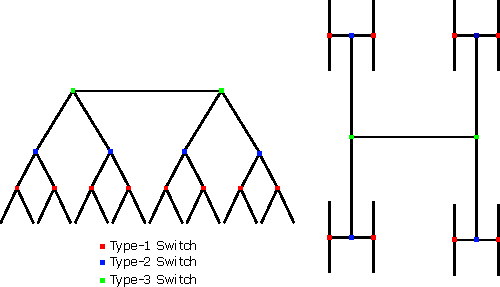
\includegraphics[width=\columnwidth]{Figures/HNoC.pdf}
   \caption{(a)A binary tree topology utilizing switches operating at different clock frequencies (b) The tree as an H-tree for better floorplanning on the FPGA}
   \label{fig:btree}
\end{figure}

\begin{figure}[t]
\centering
   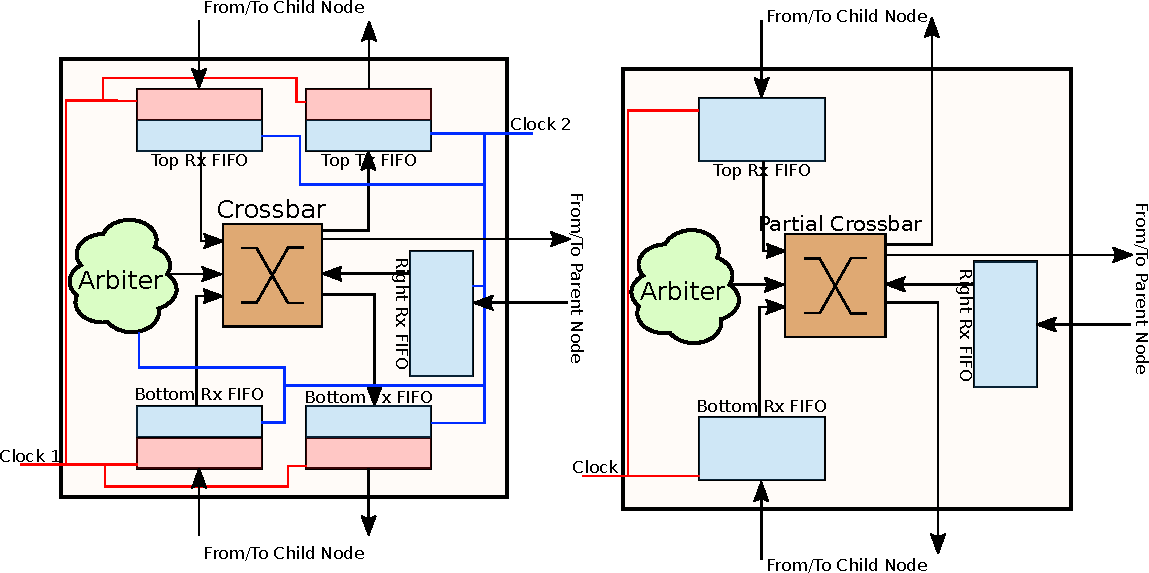
\includegraphics[width=\columnwidth]{Figures/switch1_2.pdf}
   \caption{Architecture of the different switches used in the AsyncBTree. (a) Type-1 switch used with the leaf nodes (PEs), with complete cross bar switch and asynchrnous 
   FIFOs with receive and transmit interfaces (b) Type-2 switch used in intermediate nodes with partial crossbar switch and synchronous FIFOs (c) Type-3 switches used in intermediate
   switches with partial cross bar and asynchrnous FIFOs with receive and transmit interfaces.}
   \label{fig:switchArch}
\end{figure}

\subsection{Switches}
\label{sec:switch}
AsyncBTrees use three different kinds of switches for packet routing.
The architecture of the proposed type-1 switch is as shown in Fig.~\ref{fig:switchArch}(a).
Type-1 switches are used only in the leaf nodes for directly interfacing with PEs.
The switch has separate interface for receiving and transmitting packets from two PEs and a single interface to the parent node.
Each receive and transmit interface to/from the PEs are connected to asynchronous FIFOs.
The interface to the parent node implements a single synchronous FIFO for the receive interface but no transmit FIFO.
Thus each switch contains 5 FIFOs.

Asynchronous FIFOs can operate their read and write interfaces using independent clocks.
Depth of the FIFOs are kept very low (16) to reduce the resource utilization.
The asynchronous FIFOs receive data from the downstream ports on Clock 1 signal.
The received packets are routed to the appropriate output ports by an arbitrator through a cross-bar switch.
The read side of the receive FIFO, the write side of the transmit FIFO, the arbitrator and the cross bar works on Clock 2 signal, whose frequency will be much higher than that of Clock 1.
In order to match the performance of a binary fat tree, Clock 2 frequency should be twice as that of Clock 1.

Type-1 switches implement a full cross bar, which enables loop back of packets at the switch level.
The arbitrator internally uses flit-level round-robin arbitration scheme to select the input port when more than one port requests for the same output port.
If a single input port is requesting for a particular output port, it is given the port access until all the flits are sent out.

Fig.~\ref{fig:switchArch}(b) shows the architecture of a type-2 switch.
Type-2 switches are synchronous in nature and are similar to the switches of traditional binary trees.
These switches implement only partial cross-bar switch where an in coming packet cannot be routed back to the same port.
Since these switches are used only in intermediate levels, there is no necessity to to support loop-back since they are already implemented by Type-1 switches.
This simplifies the switch design and helps in reducing resource utilization.

Type-3 switches (Fig.~\ref{fig:switchArch}(b)) are similar to type-1 switches except that they implement only a partial cross-bar similar to type-2 switches.
Type-2 and type-3 switches can be interchangeably used in the proposed architecture. 
Theoretically to match the performance of a binary fat tree, AsyncBTrees should be implementing type-3 switches at every level with increasing clock frequencies.
But in practical scenarios, doubling clock frequency at each level is not possible in FPGAs as the tree size increases.
The maximum frequency supported by modern devices are in the order of hundredes of megahertz.
Hence for practical implementations, AsyncBTrees increases the clock frequency only for alternative levels. 
Although asynchronous FIFOs can operate using same clock signal for read and write interfaces, the resource utilization of an asynchronous FIFOs is much more than its synchronous counter part for a given FIFO size.
It is because of the presence of additional circuitry for managing clock domain crossing between the read and write interfaces.
For reducing resource consumption, levels which operates on synchronous clock uses type-3 switches and levels which operate on asynchronous clock uses type-2 switches.

\subsection{Routing}
\label{sec:routing}
AyncBTree uses fixed routing based on the destination address of the packet header~\ref{fig:packet}.
The routing is flit level routing meaning each packet is expected to have the destination PE address in the packet header.
Larger packets are sent as multiple flits.
One major advantage of binary trees is the multiple packets sent from one PE to another will be always delivered in the sent order.
In other packet switched networks such as mesh or torus, the packets could be delivered in out of order depending on the routing algorithms.
In this case additional logic is required for packet reassembly and packet numbers also have to be inserted into the payload.

The routing table of each switch in AsyncBTree contains four entries corresponding to the smallest and largest PE addresses in its left sub-tree and right sub-tree.
If the destination address is with in the range of left sub-tree, it is routed left and if it is with in the range of right sub-tree the packet is sent right.
If the address is not within these ranges, the packet is routed towards the parent node.
Due to the deterministic routing policy and since the routing is at flit-level, the NoC is free of dead or livelocks.

\begin{figure}[t]
\centering
   
\includegraphics[width=\columnwidth]{Figures/pckt_structure.pdf}
   \caption{Packet structure}
   \label{fig:packet}
\end{figure}

\section{Flow control}
The current AsyncBTree implementation does not include virtual channels and flow control is achieved through at electrical signaling level.
The interface between switches as well as switches and PEs confirm to AXI4-stream interface.
Such interface also enables seamless integration of several vendor supported IP cores directly with the NoC.
As per AXI4-stream protocol, a successful data transfer happens only when the \emph{valid} signal from the transmitter and \emph{ready} signal from the receiver are asserted as shown in Fig.~\ref{axi}.
%\section{Results and Discussion}
\label{sec:result}

In this section we discuss the implementation and performance comparison of the different NoC implementations.
All designs are modeled using Verilog HDL and extensively simulated for their functional correctness.
We use the CONNECT open-source NoC platform as the fat tree, mesh and torus references~\cite{papa_connect_fpga2012}.
The designs are simulated as well as implemented with Vivado 2017.3 targeting Xilinx xc7vx690t FPGA (VC709 evaluation board).

\input Tables/SystemResource
Table~\ref{table:systemResourceConsumption} compares the resource utilization and the maximum frequency of operation for the binary tree, AsyncBTree, and fat tree for different network sizes (number of PEs).
For all implementations, the interface between PEs and the switches are kept 32-bits wide.
As expected, binary trees are least resource intensive due to their simple switch architecture.
AsyncBTree consumes 45\% to 65\% more LUTs (look-up-tables) and about 165\% more flip flops compared to the binary tree implementation.
The multiple frequencies in the AsyncBTree rows represent the maximum clock frequency supported at different tree levels.
At the lowest level (switches connected to PEs), the clock performance is better than that of binary trees but deteriorates as going higher in the hierarchy.
This could be because of the additional pipelining present inside the asynchronous FIFOs.
This also means if AsyncBTree is used as a synchronous NoC (all tree levels are clocked by a single clock source), its resource consumption and performance will be worse than a binary tree. 

Compared to AsyncBTree, fat trees consume $\sim$3.7$\times$ LUTs but less than half the number of flip flops.
AsyncBTree requires more flip flops due to the presence of asynchronous FIFOs.
For fat trees, the impact due to complex switches can be clearly seen in the clock performance, where they are not even able to achieve 200 MHz for a high-end FPGA.
Due to the low clock performance of the NoC, the PEs also have to be under-clocked in most scenarios for overall synchronous operations.
%Otherwise synchronization FIFOs have to be inserted between PEs and the NoC switches, which will further increase the resource utilization.
Considering the fact that the number of LUTs available in 7-series Xilinx FPGAs are half of that of number of flip-flops, AsyncBTree is much lite compared fat trees at the same time given more than 4$\times$ clock performance.

\input Tables/ResourceDiffConf
Table~\ref{table:NocResourceUtilisation} lists the resource utilization and clock performance of the most popular FPGA NoC topologies namely mesh and torus.
Data shows that these topologies are quite resource intensive compared to all binary tree configurations, especially the number of LUTs.
In terms of clock performance, for larger NoC configurations, they perform better than fat trees but inferior to traditional binary trees and the proposed AsyncBTrees.

Fig.~\ref{fig:tput} and~\ref{fig:latency} compares the throughput and latency of the three implementations with different NoC sizes for different traffic patterns such as random, tornado and reverse~\cite{Bahn2008}.
The different patterns are generated based on how the destination addresses as generated for each data packet.
In each case, the PE to switch interface is clocked at the lowest frequency supported among the three implementations.
For AsyncBTree upper levels are clocked at double the frequency of lower levels, but limited by maximum supported frequency given in Table~\ref{table:systemResourceConsumption}.
It could be seen that for NoC size up to 8 PEs, AsyncBTree performance is better than or comparable to that of fat trees.
For larger tree sizes, fat trees perform better since the clock frequencies cannot be scaled beyond a limit.
If PEs run at lower clock frequencies ($\sim$50 MHz), AsyncBTree can provide better performance for NoC with up to 16 PEs. 

Fig.~\ref{fig:tputmax} and~\ref{fig:latmax} compares the throughput and latency when each implementation is running at its maximum supported frequency.
Again for smaller NoC sizes binary tree and AsyncBTree out performs fat tree for random traffic pattern.
But for larger NoC sizes fat trees are clearly advantageous.
Fig.~\ref{fig:tputmax}(a) also shows the performance of mesh topology, which is the most popular NoC topology, compared to different tree topologies.
Again for smaller NoC sizes (8 or less) AsyncTree performance is better.
Several FPGA-based multi-processor systems have 8 core or less thus AsyncBTree could be much suitable for their implementation.

Fig.~\ref{fig:tputPerf} compares the performance of each NoC compared to their resource utilization.
The total number of resources is calculated by adding the number of LUTs with the scaled number of flip-flops.
The number of flip-flops is multiplied by a factor of 0.5 since in Xilinx 7-series FPGAs there are twice the number of flip-flops compared to LUTs in every logic slice.
Synchronous binary trees clearly have an upper hand in this regard.
AsyncBTree give moderately high throughput by consuming relatively less resources.
But for larger NoC size, mesh topology is still the suitable candidate.


\begin{figure}[t]
\centering
   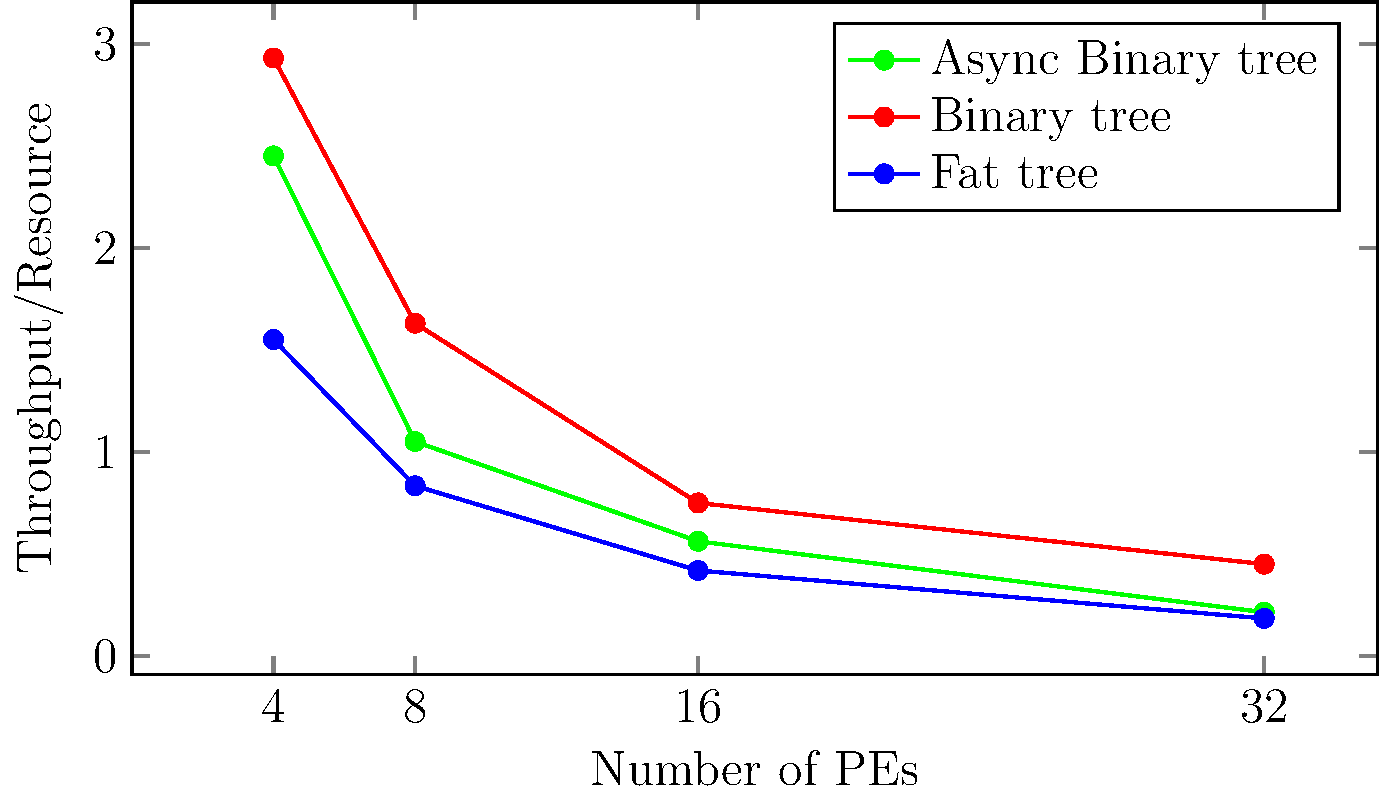
\includegraphics[width=\columnwidth]{Data/tputVsCost.pdf}
   \vspace{-5mm}
   \caption{Throughput vs cost}
   \vspace{-5mm}
      \label{fig:tputPerf}
\end{figure}

%\section{Conclusion}
\label{sec:conclusion}
In this paper we discussed the implementation of an asynchronous binary tree based NoC architecture targeting FPGA implementation.
Analysis shows that FPGA archtiecture specific optimization can provide high clock performance and low resource consumption for such implementation compared to traditional fat-tree based implementations.
It also shows the advantage of fixed size interface to PEs compared to variable size interface when targeting the NoC for partial reconfiguration.
Implementation of the proposed architecture is provided as an open source enabling other researchers to verify its functionality and to use in practical NoC-based applications~\cite{hnoc}.
In the future we will be anayzing the effect of GALS-based implementation of other network topologies when targeting FPGA implementations.



%\bibliographystyle{IEEEtran}
%\bibliography{nocs} 

\end{document}
